\documentclass[12pt,a4paper]{article}
\usepackage[utf8]{inputenc}
\usepackage[T1]{fontenc}
\usepackage[francais]{babel}
\usepackage{amsmath}
\usepackage{amsfonts}
\usepackage{amssymb}
\usepackage{graphicx}
\usepackage[top=2.00cm]{geometry}
\usepackage{titlesec}
\usepackage{multicol}
\usepackage{bigcenter}
\usepackage{capt-of}
%%modif des titres de section diminuer la taille
\graphicspath{{C:/Users/Sylvain/AppData/Roaming/texstudio/templates/user/}}
\renewcommand{\thesection}{\Roman{section}}
\titleformat{\section}
{\normalfont\bfseries\Large\scshape}{\thesection}{1em}{}
\titleformat{\subsection}
{\normalfont\bfseries\large}{\thesubsection}{1em}{}
\DeclareMathOperator{\sinc}{sinc}
\makeatletter
\def\@maketitle{
	
	\begin{center}
		% NoLogo
		% \vspace*{+2cm}
		
		% Corner Logo
		% \begin{flushright}
		%  
\includegraphics[width=40mm]{logo_corner}\\[4ex]
		% \end{flushright}
		
		% Top Logo
		
\includegraphics[scale=0.3]{logo_top}
		
		
		{\LARGE \@title }\\[4ex]
		{\large \@author}\\[4ex]
		{\large \@date}\\[8ex]
		\rule{\linewidth}{0.4pt}
	\end{center}
}
\makeatletter

\author{CHARNAY Valentin, FINOT Sylvain}
\title{Compte rendu de TP :\\[4pt] \scshape Diffraction}

\date{\today}
\begin{document}
	\maketitle
%	\section{Théorie}
	\section{Étude de la réponse impulsionnelle d'un système stigmatique}
	On utilise dans cette partie un laser rouge de longueur d'onde $\lambda=632,8$nm en guise de source monochromatique. On étudie les figures de diffraction obtenues avec différentes pupilles diffractantes.
	\subsection{Diffraction par un bord}
	On se sert ici d'un bord de lame de rasoir comme objet diffractant. Il est proposé dans l'énoncé de se servir de miroirs pour augmenter la distance lame-écran. Nous avons choisi de ne pas utiliser les miroirs que l'on avait à notre disposition, nous avons donc directement allongé la distance lame-écran en se mettant de part et d'autre de la salle de TP.
	
	Sur la figure obtenue, on remarque un pic d'intensité au centre puis des petites raies moins lumineuses. À noter que nous avons installé le détecteur perpendiculaire à la lame de rasoir. Pour un bord horizontal, on obtient des raies horizontales de moins en moins lumineuses en s'éloignant verticalement. 
	\begin{center}
		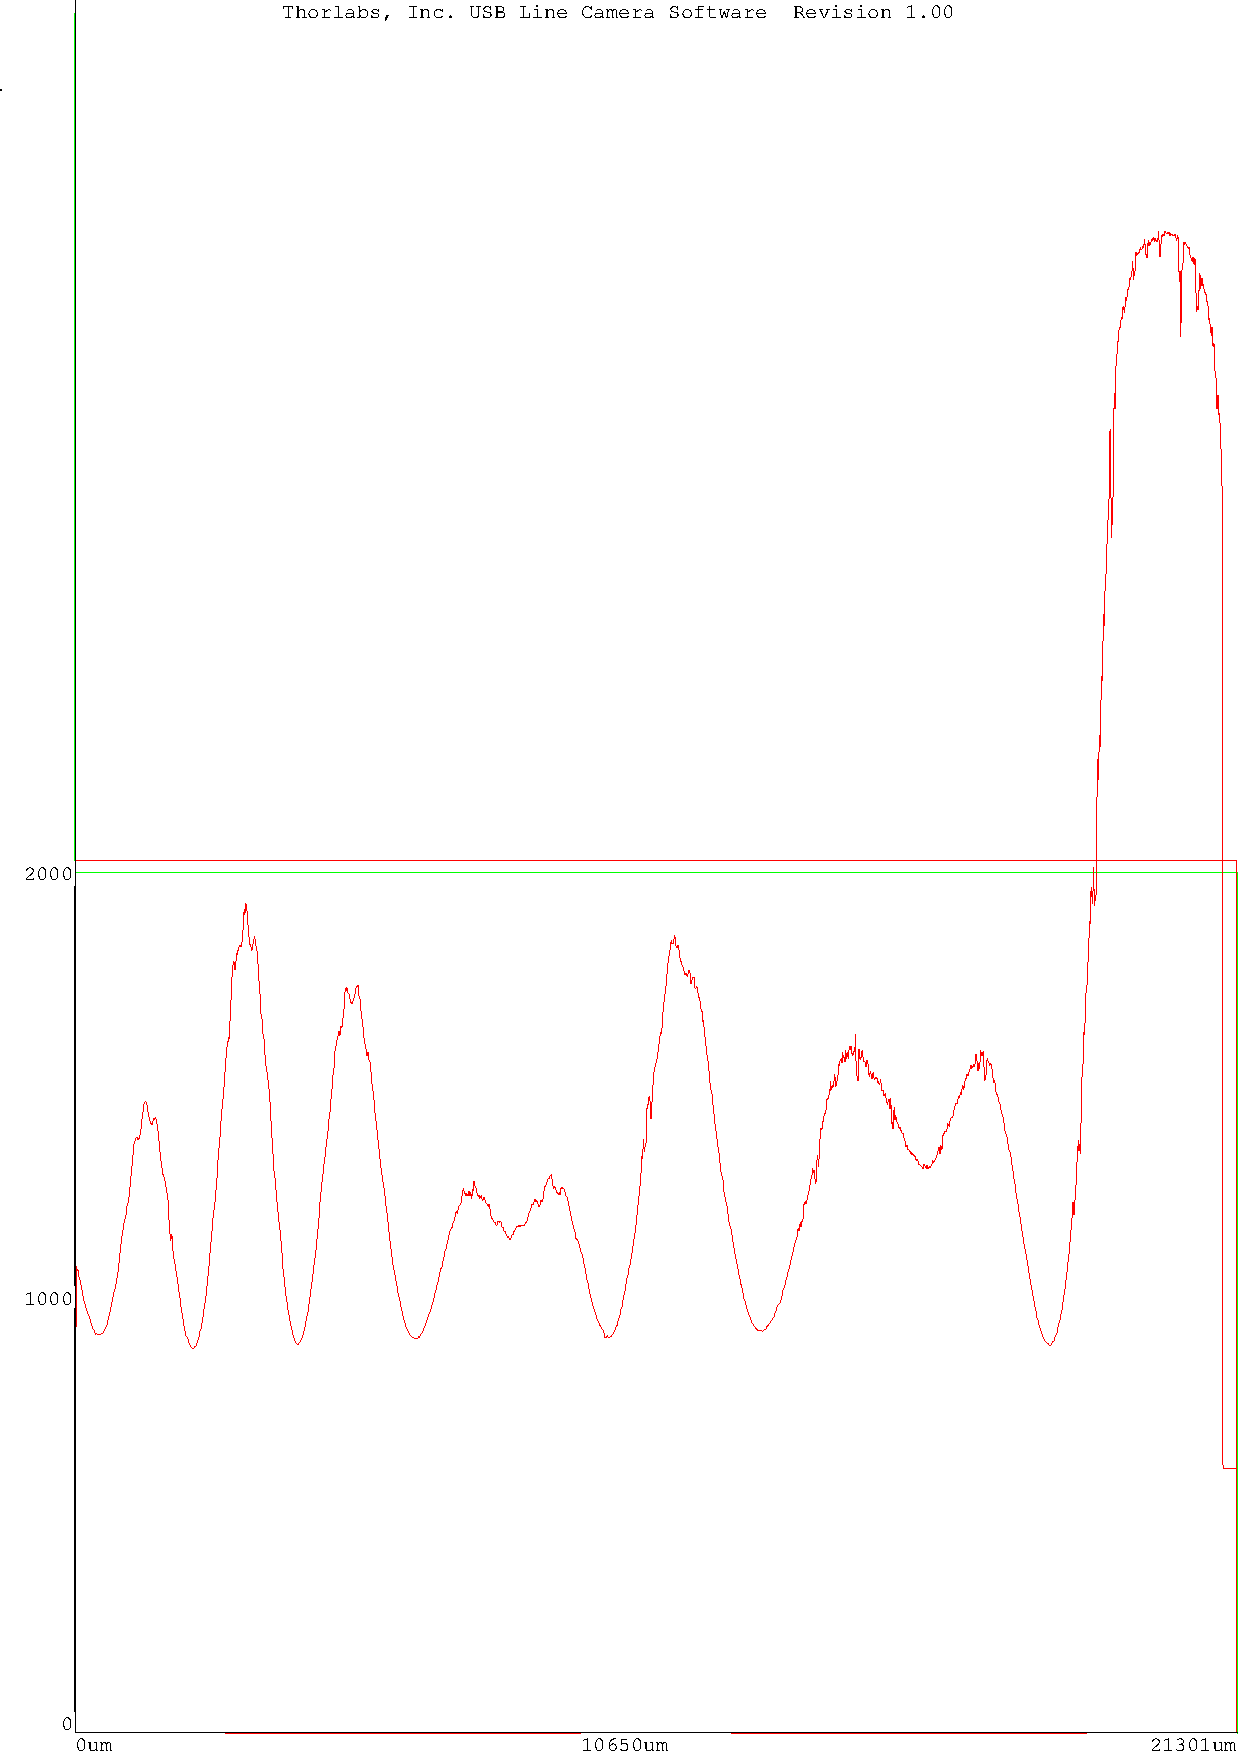
\includegraphics[scale=0.45]{res/rasoir}
	\end{center}
	\subsection{Diffraction par un trou}
	En diffractant la lumière du laser par un trou, on obtient une figure ayant l'allure d'un sinus cardinal au carré (voir ci-dessous). Pour être exact, il s'agit d'une fonction de Bessel.\\
	L'intensité lumineuse est donnée par :
	$$I=I_0 \left( \dfrac{2J_1(\pi u)}{\pi u}\right) \quad \text{où}\quad u\equiv\dfrac{4\alpha R}{\lambda}$$
	La fonction J$_1$ est une fonction de Bessel qui s'annule pour $u\approx k+1/4$
	Regardons si on retrouve cette condition dans nos mesures.\\
	Dans les conditions de mesures, on a : \\
	
	
	\bgroup
	\setlength{\tabcolsep}{1.5em}
	\def\arraystretch{1.25}
	\begin{tabular}{lll}
		\hline
		\hline
		R &  rayon du trou & 50$\mu m$  \\ 
		% \hline 
		D & distance trou-écran &  11,6cm\\ 
		% \hline 
		dx& Abscisse horizontale d'un minimum &  3752$\mu m$\\ 
		$\lambda$& longueur d'onde &  632,8nm\\ 
		\hline 
		\hline
	\end{tabular}  
	\egroup
	
	\begin{center}
		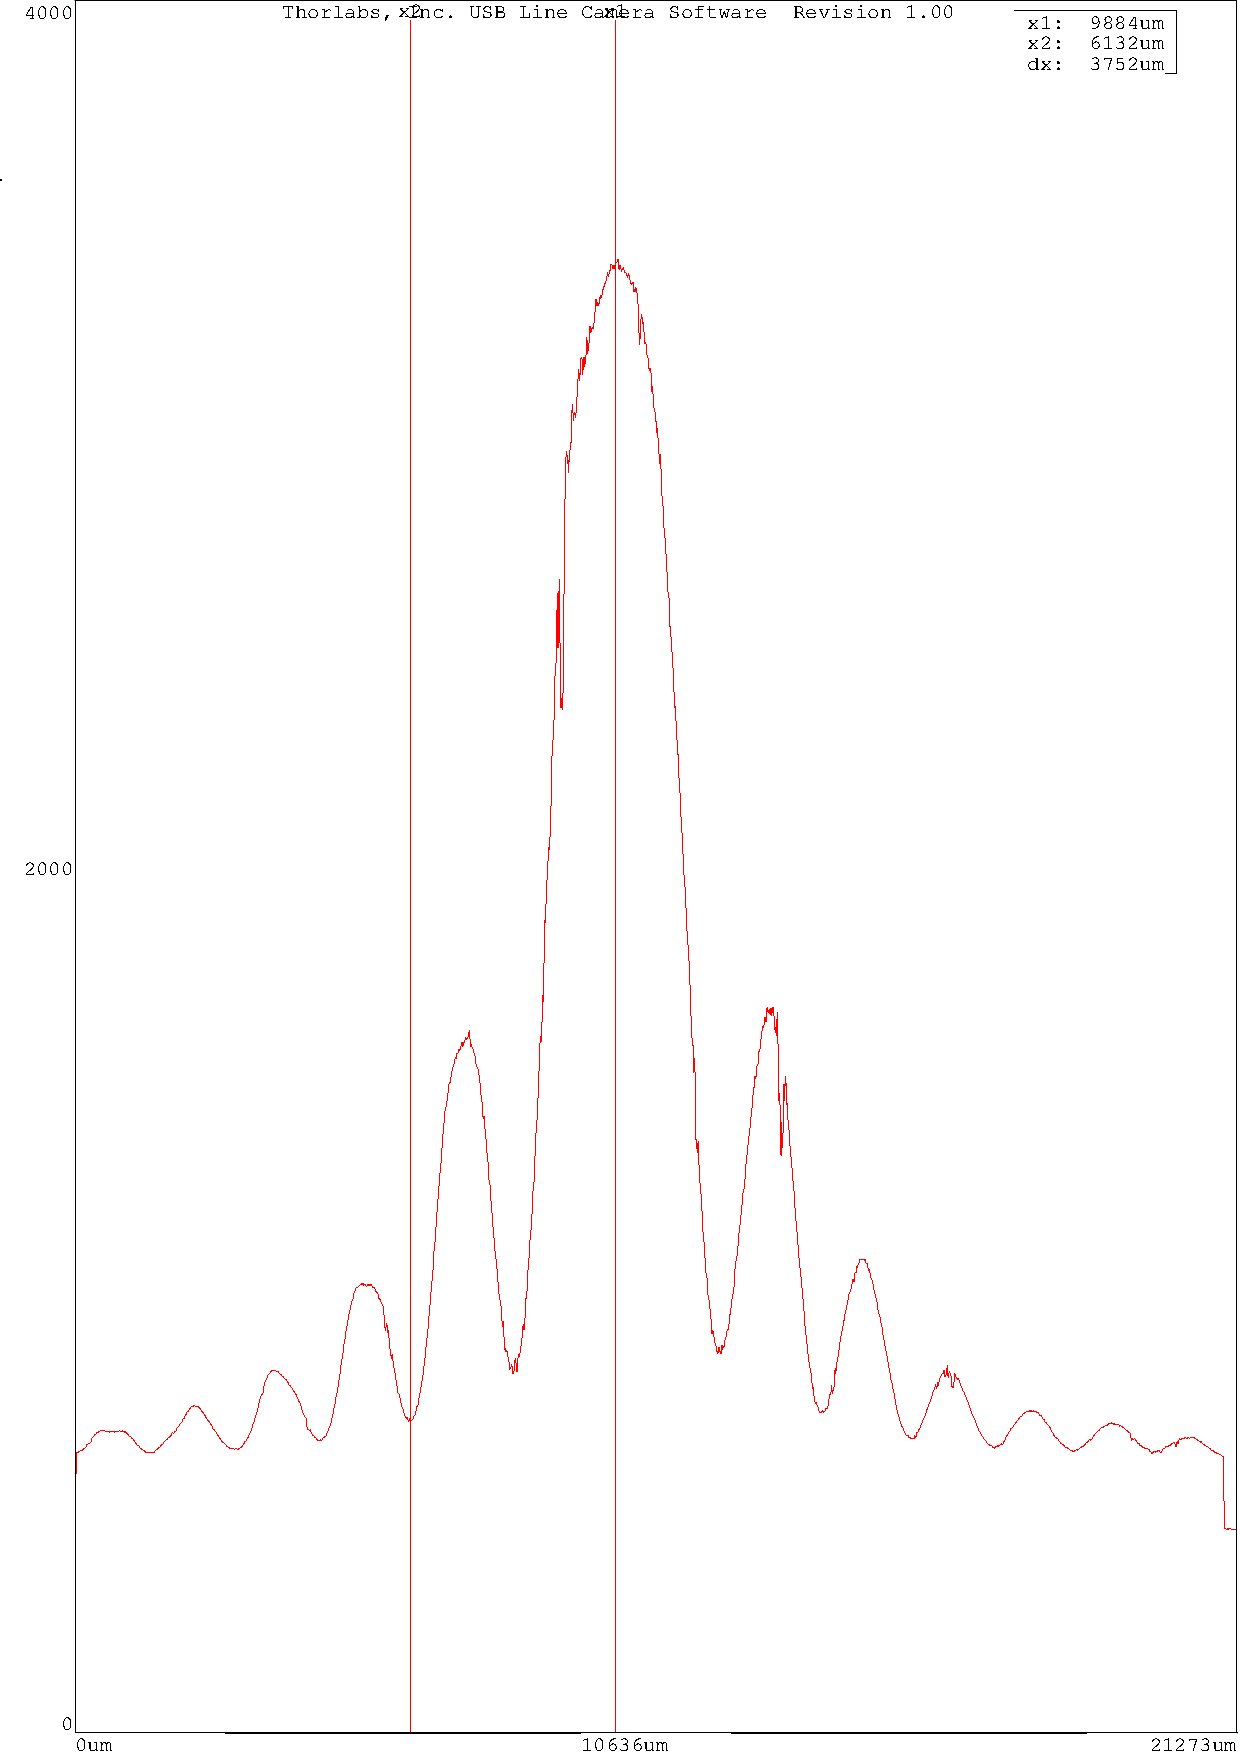
\includegraphics[scale=0.35]{res/trou2}
	\end{center}
	Théoriquement on a $\tan\alpha=\dfrac{dx}{D}$ or $D\gg dx$ on peut donc faire l'approximation suivante : $\alpha\approx\dfrac{dx}{D}$.
	\bgroup
	\addtolength{\jot}{4pt}
	\begin{align*}
	u&=\dfrac{4\alpha R}{\lambda}\\
	&\approx\dfrac{4 \left(\dfrac{dx}{D}\right) R }{\lambda}\\
	&\approx\dfrac{4\times50.10^{-6}\times3752.10^{-6}}{632,8.10^{-9}\times11,6.10^{-2}}\\
	&\approx10,22
	\end{align*}
	\egroup
	On retrouve le k+1/4 avec k=10\\
	\textbf{Remarques :}
	\begin{itemize}
		\item  Bien que nous ayons pris le deuxième minimum, le k trouvé est plus grand.
		\item  Si on déplace le trou parallèlement à l'axe optique, on joue sur la taille des inter-franges.
	\end{itemize}
	\subsection{Diffraction par une fente, un fil}
	Nous n'avons pas trouvé de fil de même épaisseur qu'une fente. Cependant en prenant une fente d'épaisseur approximativement égale à celle d'un fil (même ordre de grandeur), on observe que les figures de diffraction sont identiques (à l'œil nu).
	Ce résultat s'explique par le théorème de Babinet qui énonce que les figures de diffraction de deux surfaces complémentaires sont identiques.\\
	\begin{bigcenter}
		\begin{multicols}{2}
			\bgroup
			%  \centering
			\includegraphics[scale=0.075,trim=0 40cm 15cm 40cm,clip]{res/"fil 20170207_162645"}
			\captionof{figure}{Diffraction par un fil}
			\egroup
			
			\columnbreak
			\vfill
			\bgroup
			\includegraphics[width=\linewidth,trim=20cm 5cm 0 22cm,clip]{res/"fente 20170207_163022"}
			\captionof{figure}{Diffraction par une fente}
			\egroup
		\end{multicols}
	\end{bigcenter}
	
	\subsection{Diffraction par deux réseaux croisés}
	Lorsque l'on diffracte le faisceau d'un laser par deux réseaux croisés, on obtient la figure suivante :\\
	\begin{bigcenter}
	\begin{multicols}{2}
			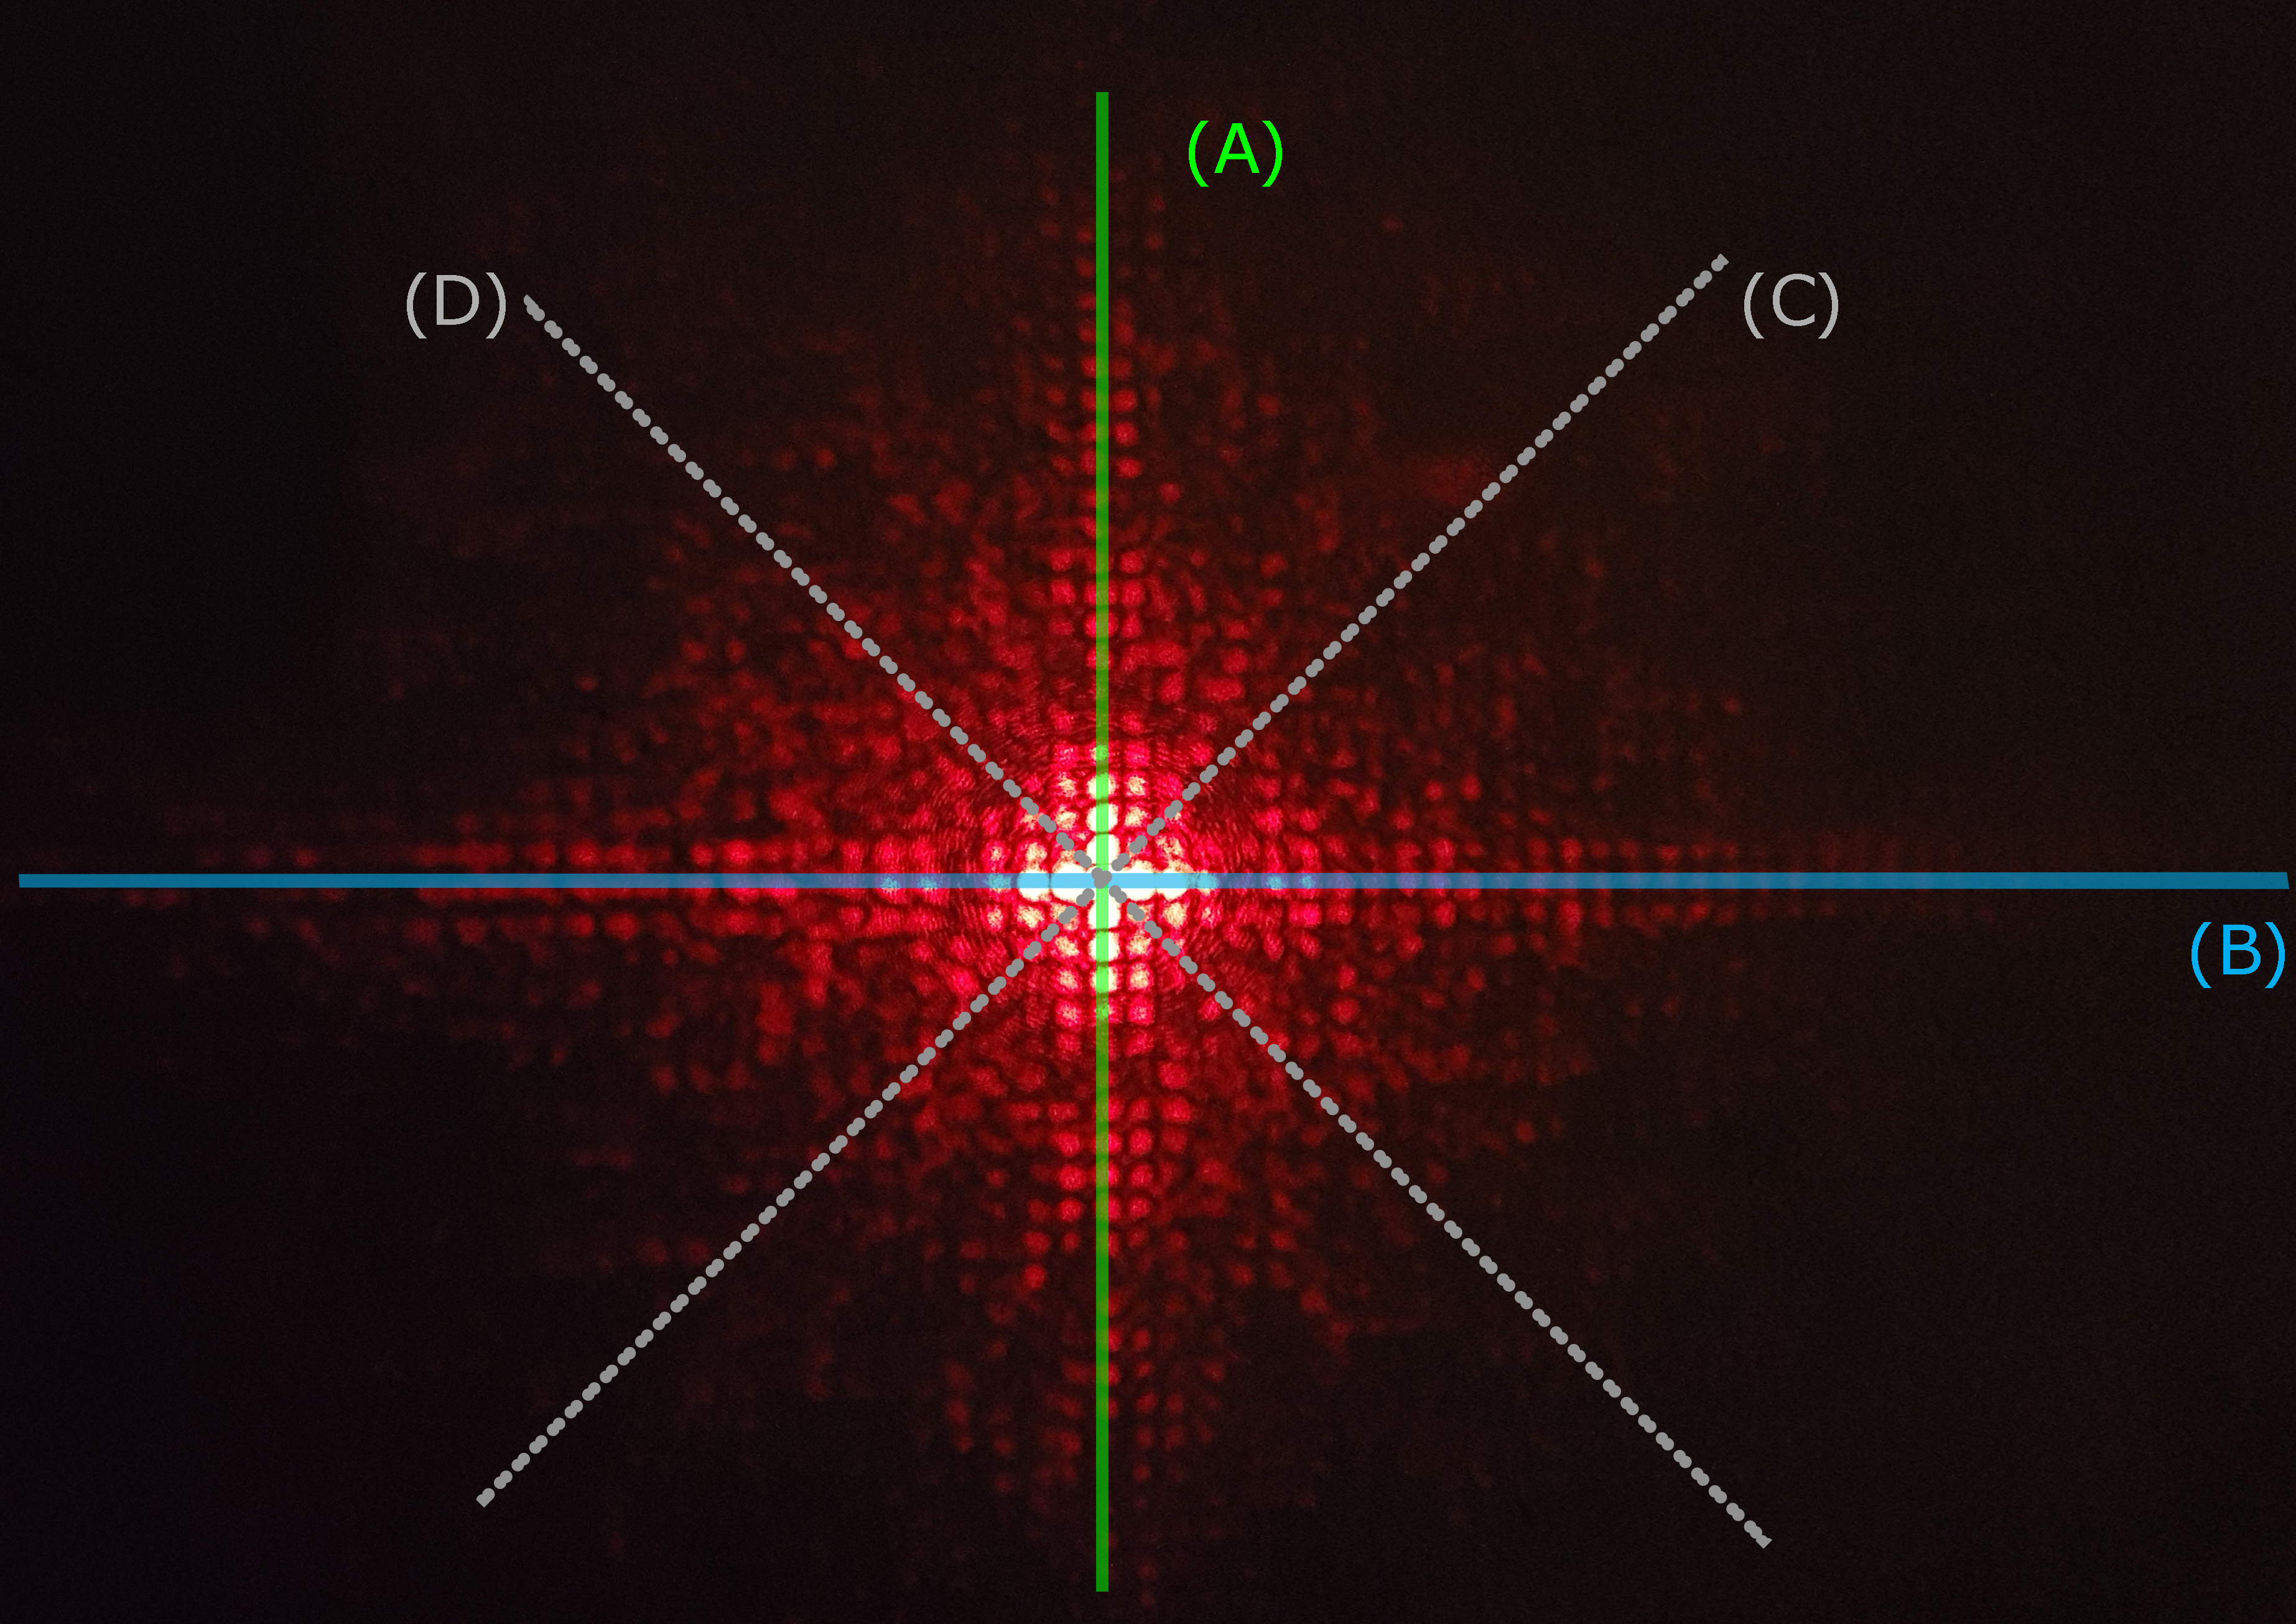
\includegraphics[width=\linewidth]{res/reseaux_axes}
			\captionof{figure}{Diffraction par réseaux croisés}
			\columnbreak
			\includegraphics[width=\linewidth, trim= 25cm 20cm 25cm 20cm,clip]{"res/reseaux"}
			\captionof{figure}{Diffraction par réseaux}
	\end{multicols}
	\end{bigcenter}
%	\begin{figure}[h]
%		\centering
%		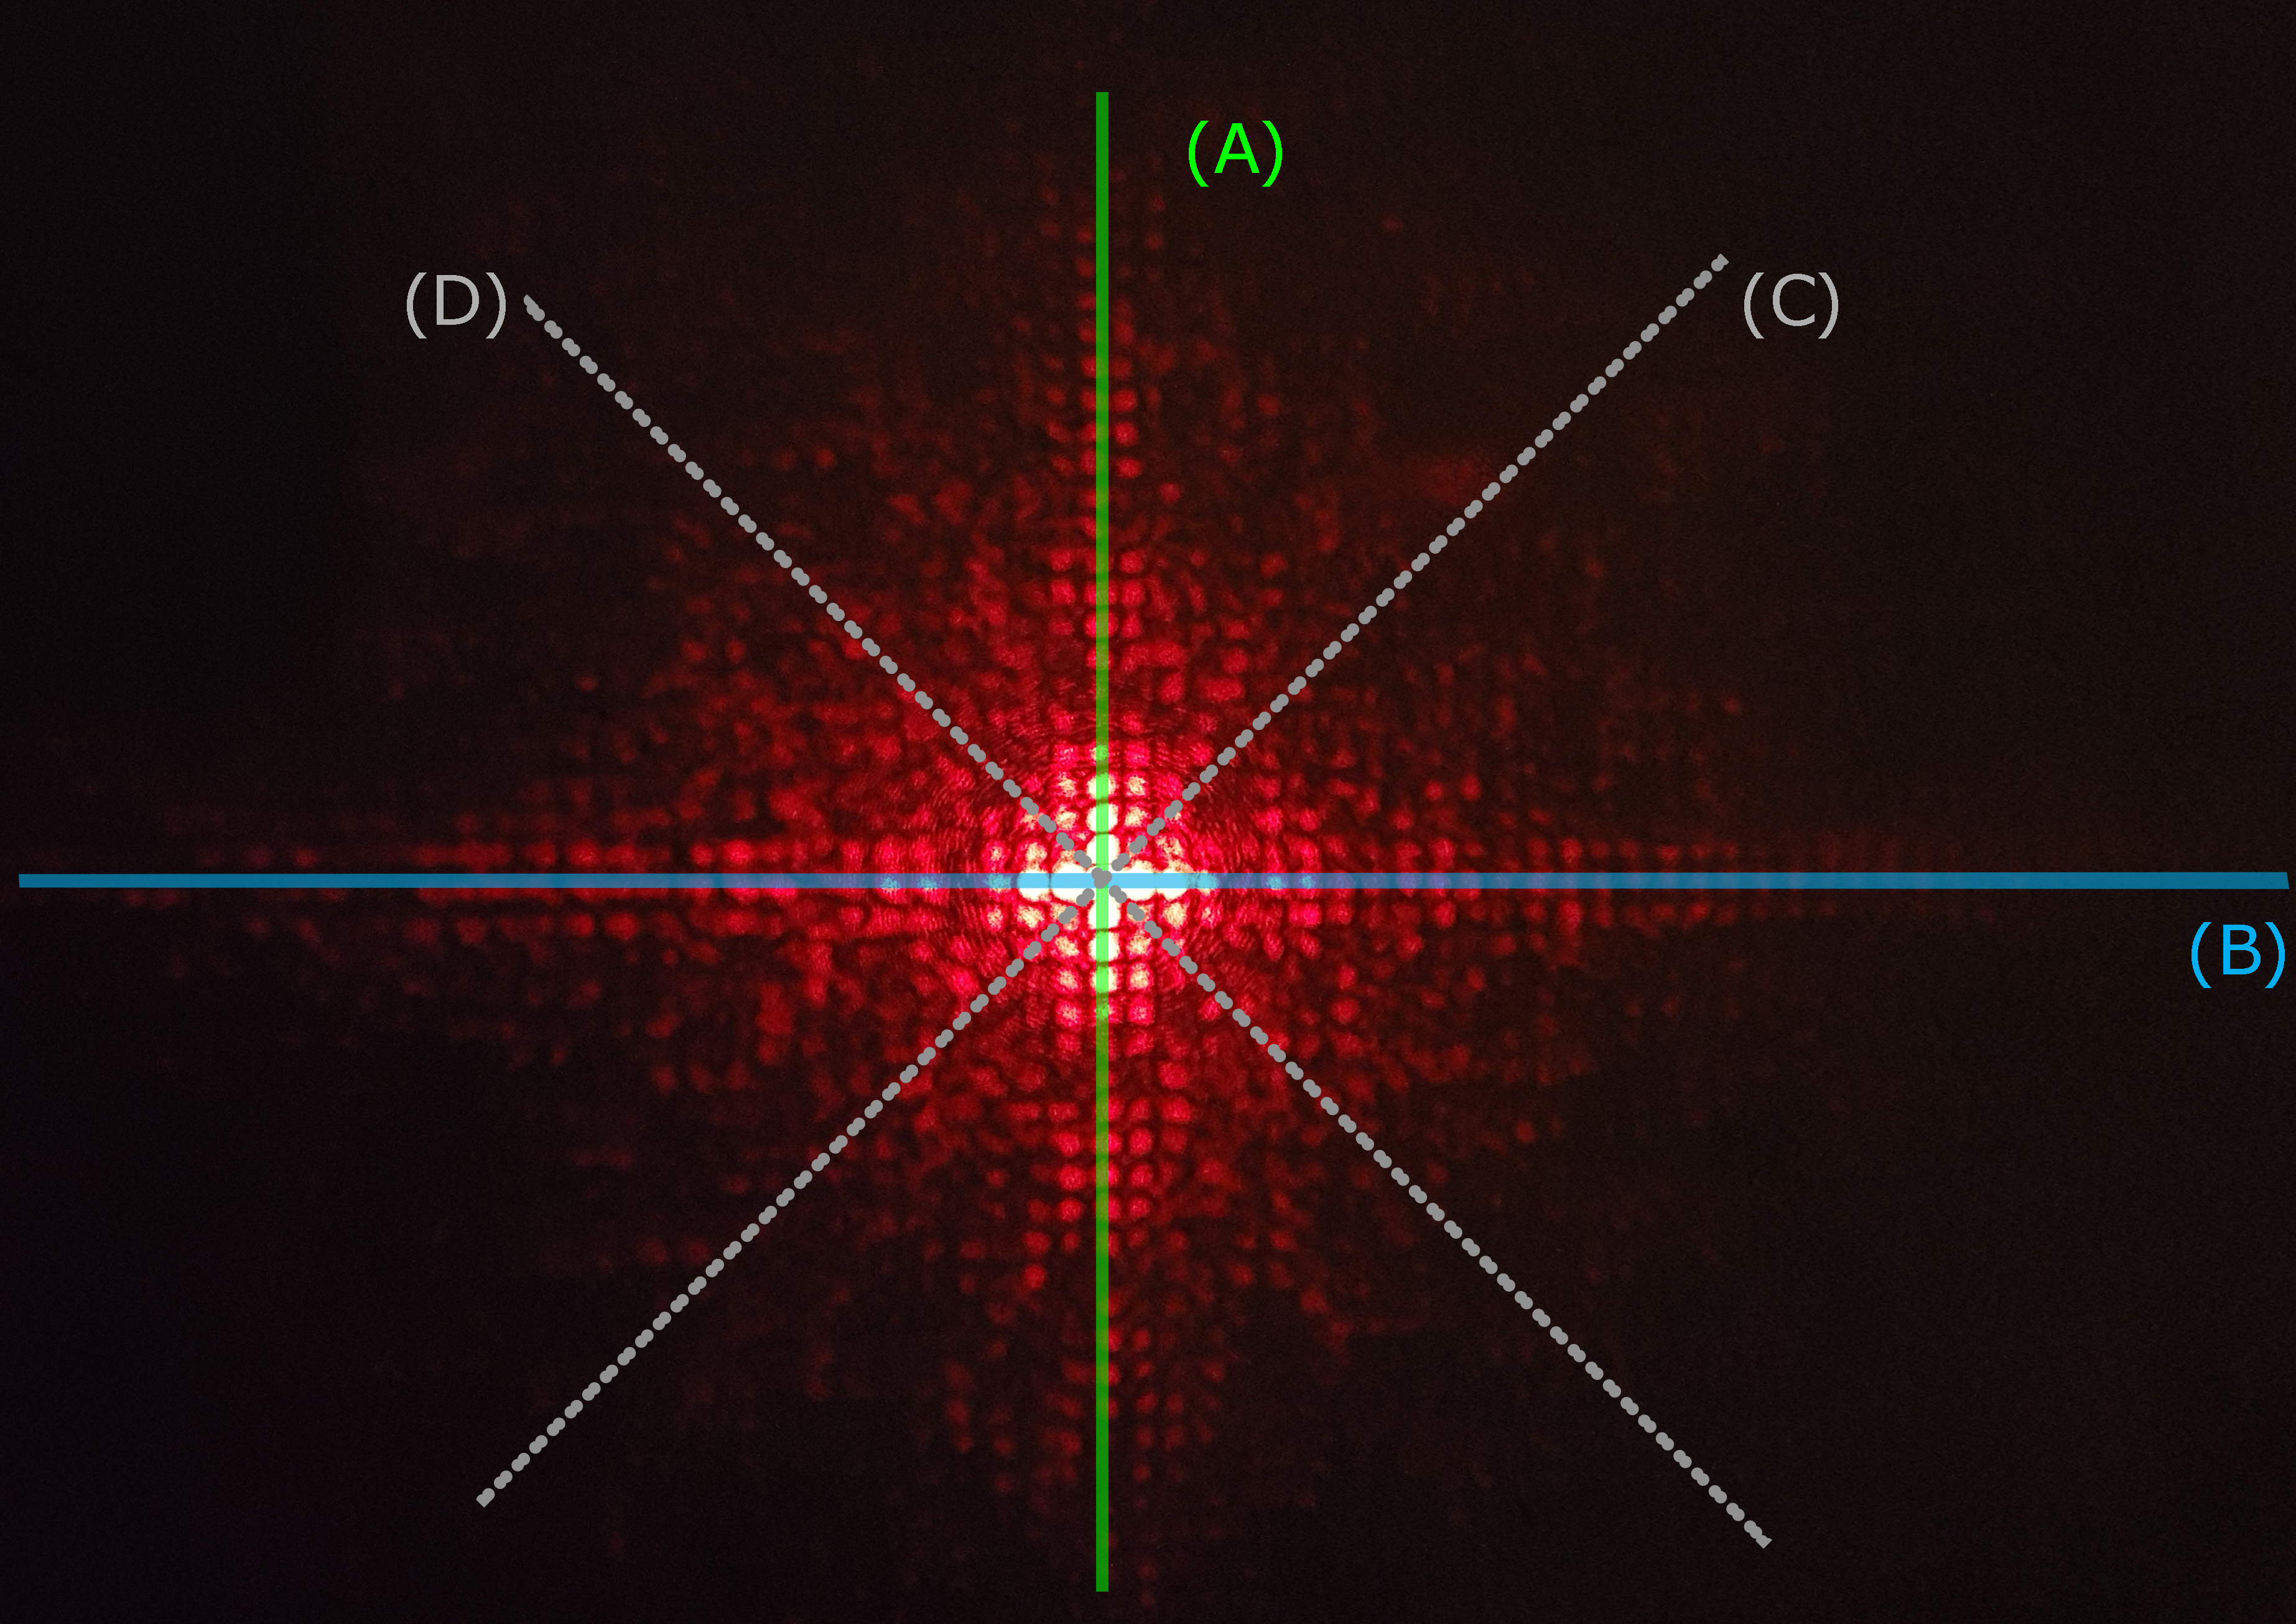
\includegraphics[scale=0.08]{res/reseaux_axes}
%		\caption{Diffraction par réseaux croisés}
%	\end{figure}
	
	On remarque différents axes de symétrie:
	\begin{itemize}
		\item L'axe (A)
		\item L'axe (B)
		\item Les axes (C) et (D). On peut émettre l'hypothèse que ce sont des axes de symétrie que si les pas des réseaux horizontaux et verticaux sont identiques.
	\end{itemize}
	\subsection{Diffraction par deux fentes parallèles : frange d'Young}
	Lorsque l'on réalise la diffraction par deux fentes d'Young, l'intensité observée sur l'écran est donnée par :
	$$I(\theta)=4I_0\sinc^2\left( {\dfrac{\pi a \theta}{\lambda}}\right) \cos^2\left(\dfrac{\pi l \theta}{\lambda}\right)$$
	En relevant l'intensité au capteur, on obtient la figure suivante:
	\begin{figure}[h]
		\centering
		\includegraphics[scale=0.5]{"res/Young OK"}
		\caption{Franges d'Young}
	\end{figure}
	
	On observe bien l'enveloppe en $\sinc^2$, caractéristique du phénomène de diffraction. A l'intérieur de cette enveloppe, on remarque des oscillations (terme en $\cos^2$). Ces oscillations sont dues aux interférences entre les deux fentes.
	
	La figure obtenue est donc le résultat de la superposition d'un phénomène de diffraction (fentes fines) et d'interférences.\\
	
	En s'intéressant au terme en $\cos^2(...)$ (représentant les oscillations à l'intérieur de l'enveloppe en $\sinc$) on peut retrouver la distance entre les deux fentes. Pour cela on cherche une relation liant position d'un minimum et $l$.
	
%	\pagebreak
	On regarde à quelle condition on a :
	\begin{align*}
	&\cos^2\left(\dfrac{\pi l \theta}{\lambda}\right)=0\\
	\iff& \dfrac{\pi l \theta}{\lambda}=n \pi+\dfrac{\pi}{2}\\
	\iff& \dfrac{l x}{D\lambda}=n+\dfrac{1}{2}\\
	\iff& x_n=(n+\dfrac{1}{2})\cdot\dfrac{D\lambda}{l}
	\end{align*}
	On note $i$ la longueur entre deux minimum consécutifs.
	\begin{align*}
	i&=x_{n+1}-x_{n}\\
	&=((n+1+\dfrac{1}{2})-(n+\dfrac{1}{2}))\dfrac{D\lambda}{l}\\
	i&=\dfrac{\lambda D}{l}
	\end{align*}
	On peut donc mesurer la distance entre les fentes en mesurant la distance entre chaque minimum du $\cos^2$. Pour être plus précis, on mesure plusieurs $i$ pour en faire la moyenne. Les mesures se font dans la tache centrale pour faciliter la lecture. 
	%On peut facilement trouver la condition pour obtenir un minimum. Pour cela on calcul la différence de marche à la sortie des fentes.
	%Sur le schéma si dessous, il suffit d'exprimer la longueur des traits rouges
	%\begin{align*}
	% \delta &=H_2O_2-O_1H_1\\
	%   &=l(\sin\theta-\sin \theta')\\
	%\end{align*}
	%\begin{center}
	% \includegraphics[scale=1,trim= 0 3cm 3cm 2cm,clip]{"res/Schema Young"}
	%\end{center}
	\vspace*{+1em}
	\begin{multicols}{2}
		\noindent
		\begin{align*}
		i&=\dfrac{\lambda D}{l}\\
		\iff l &= \dfrac{\lambda D}{i}\\
		l&=\dfrac{632,8.10^{-9}\cdot 32,6.10^{-2}}{\left(\dfrac{4970}{8}\right)10^{-6}}\\
		&=0,33\pm 0,01mm
		\end{align*}
		\columnbreak
		\vfill
		\begin{tabular}{lll}
			D & Distance fentes-écran & 32,6$\pm$0,3cm\\
			$\lambda$ & Longueur d'onde du laser & 632,8nm\\
			i & Inter-franges & $\dfrac{4970.10^{-6}}{8}$m
		\end{tabular}
	\end{multicols}
La valeur trouvée par application numérique correspond à la valeur indiquée sur les fentes (0,3mm).\\
\underline{Remarque :} l'incertitude est peut être plus importante que celle calculée ici. Nous n'avons pas considérer la précision du capteur.
\subsection{Conclusion}

Tous les montages que nous avons vu permettent de mettre en avant l'aspect ondulatoire de la lumière. L'optique géométrique seule ne permet pas d'expliquer la diffraction ni le phénomène d'interférences que nous avons rencontré dans ce TP.
\end{document}

